\scanpage{29}
\textcircled{2} Cas où $M$ est un $\mathbf Z_p$-module

Notons d'abord qu'il existe des $k$ arbitrairement grands tels que $c_{i,k-i}\in\mathbf Z_p^*$ i.e. $c_{i,k-i}\not\equiv0\ (p)$. Posons $k-i=j$, il suffit de prendre $j=p^\varepsilon$, avec $\varepsilon$ tel que $p^\varepsilon>i$, donc $k=i+p^\varepsilon$. Cela montre l'unicité de $\xi$, car si $k_0$ est tel que $c_{i,k_0-i}\in\mathbf Z_p^*$, on aura
\[
\deleted{\unsure{(\alpha)|(2)}}\qquad\xi=c_{i,k_0-i}^{-1}\xi_{k_0}
\]
Considérons alors le système des
\[
\deleted{\unsure{(\beta)|(3)}}\qquad\xi'_k=c_{i,k-i}\xi,
\]
on voit de suite \deleted{\unsure{ainsi que}} que \deleted{\unsure{on}} $(\xi'_k)_{k\geq N}$ satisfait les conditions (1), (où on substitue $\xi'_k$ à $\xi_k$), et $\xi'_{k_0}=\xi_{k_0}$, donc posons
\[
\eta_k=\xi'_k-\xi_k,
\]
\deleted{les} $(\eta_k)_{k\geq N}$ satisfait encore (1), et de plus $\eta_{k_0}=0$. Il suffit de prouver alors $\eta_k=0$, \deleted{\unsure{d'où}} $\forall k\geq N$. Donc on est ramené au

\uline{Corollaire} Si $(\xi_k)_{k\geq N}$ \deleted{est} satisfait (1), et \inserted{si} de plus \deleted{$\unsure{(1')}$} \unsure{on a donné} un $k_0\geq N$ tel que
\figure{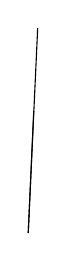
\begin{tikzpicture}\draw (0,0) -- (-0.12,-2.6);\draw (-0.05,-1.05) -- (-0.12,-2.6);\end{tikzpicture}}
\[
(1')\qquad\xi_{k_0}=0
\]
\[
(3)\qquad c_{i,k_0-i}\not\equiv0\ (p)
\]
alors $\xi_k=0\qquad\forall k>N$.
\mspage{28}
